\documentclass[aspectratio=169]{../latex_main/tntbeamer}  % you can pass all options of the beamer class, e.g., 'handout' or 'aspectratio=43'
\usepackage{dsfont}
\usepackage{bm}
\usepackage[english]{babel}
\usepackage[T1]{fontenc}
%\usepackage[utf8]{inputenc}
\usepackage{graphicx}
\graphicspath{ {./figures/} }
\usepackage{algorithm}
\usepackage[ruled,vlined,algo2e,linesnumbered]{algorithm2e}
\usepackage{hyperref}
\usepackage{booktabs}
\usepackage{mathtools}

\usepackage{amsmath,amssymb}

\DeclareMathOperator*{\argmax}{arg\,max}
\DeclareMathOperator*{\argmin}{arg\,min}

\usepackage{amsbsy}
\newcommand{\vect}[1]{\bm{#1}}
%\newcommand{\vect}[1]{\boldsymbol{#1}}

\usepackage{pgfplots}
\pgfplotsset{compat=1.16}
\usepackage{tikz}
\usetikzlibrary{trees} 
\usetikzlibrary{shapes.geometric}
\usetikzlibrary{positioning,shapes,shadows,arrows,calc,mindmap}
\usetikzlibrary{positioning,fadings,through}
\usetikzlibrary{decorations.pathreplacing}
\usetikzlibrary{intersections}
\pgfdeclarelayer{background}
\pgfdeclarelayer{foreground}
\pgfsetlayers{background,main,foreground}
\tikzstyle{activity}=[rectangle, draw=black, rounded corners, text centered, text width=8em]
\tikzstyle{data}=[rectangle, draw=black, text centered, text width=8em]
\tikzstyle{myarrow}=[->, thick, draw=black]

% Define the layers to draw the diagram
\pgfdeclarelayer{background}
\pgfdeclarelayer{foreground}
\pgfsetlayers{background,main,foreground}

% Requires XeLaTeX or LuaLaTeX
%\usepackage{unicode-math}

\usepackage{fontspec}
%\setsansfont{Arial}
\setsansfont{RotisSansSerifStd}[ 
Path=../latex_main/fonts/,
Extension = .otf,
UprightFont = *-Regular,  % or *-Light
BoldFont = *-ExtraBold,  % or *-Bold
ItalicFont = *-Italic
]
\setmonofont{Cascadia Mono}[
Scale=0.8
]

% scale factor adapted; mathrm font added (Benjamin Spitschan @TNT, 2021-06-01)
%\setmathfont[Scale=1.05]{Libertinus Math}
%\setmathrm[Scale=1.05]{Libertinus Math}

% other available math fonts are (not exhaustive)
% Latin Modern Math
% XITS Math
% Libertinus Math
% Asana Math
% Fira Math
% TeX Gyre Pagella Math
% TeX Gyre Bonum Math
% TeX Gyre Schola Math
% TeX Gyre Termes Math

% Literature References
\newcommand{\lit}[2]{\href{#2}{\footnotesize\color{black!60}[#1]}}

%%% Beamer Customization
%----------------------------------------------------------------------
% (Don't) Show sections in frame header. Options: 'sections', 'sections light', empty
\setbeamertemplate{headline}{empty}

% Add header logo for normal frames
\setheaderimage{
	% 
\includegraphics[height=\logoheight]{figures/TNT_darkv4.pdf}
	
\includegraphics[height=\logoheight]{../latex_main/figures/luh_logo_rgb_0_80_155.pdf}
	% 
\includegraphics[height=\logoheight]{figures/logo_tntluh.pdf}
}

% Header logo for title page
\settitleheaderimage{
	% 
\includegraphics[height=\logoheight]{figures/TNT_darkv4.pdf}
	
\includegraphics[height=\logoheight]{../latex_main/figures/luh_logo_rgb_0_80_155.pdf}
	% 
\includegraphics[height=\logoheight]{figures/logo_tntluh.pdf}
}

% Title page: tntdefault 
\setbeamertemplate{title page}[tntdefault]  % or luhstyle
% Add optional title image here
%\addtitlepageimagedefault{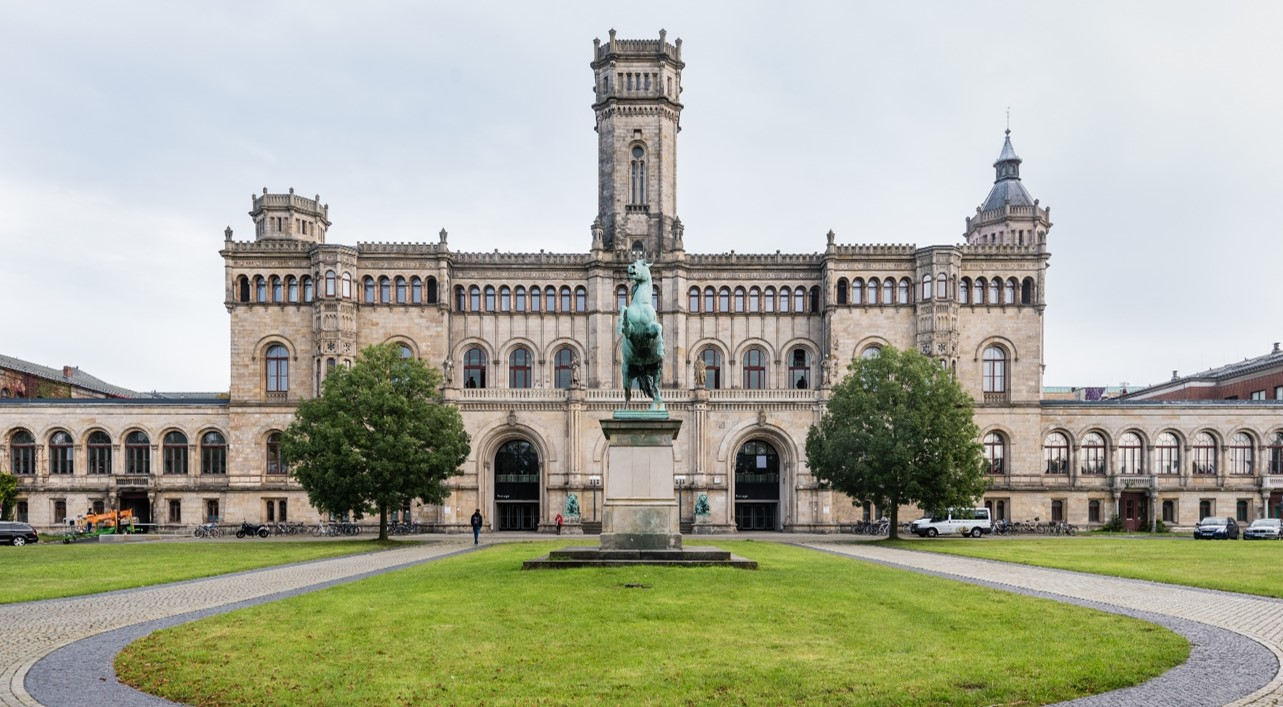
\includegraphics[width=0.65\textwidth]{figures/luh_default_presentation_title_image.jpg}}

% Title page: luhstyle
% \setbeamertemplate{title page}[luhstyle]
% % Add optional title image here
% \addtitlepageimage{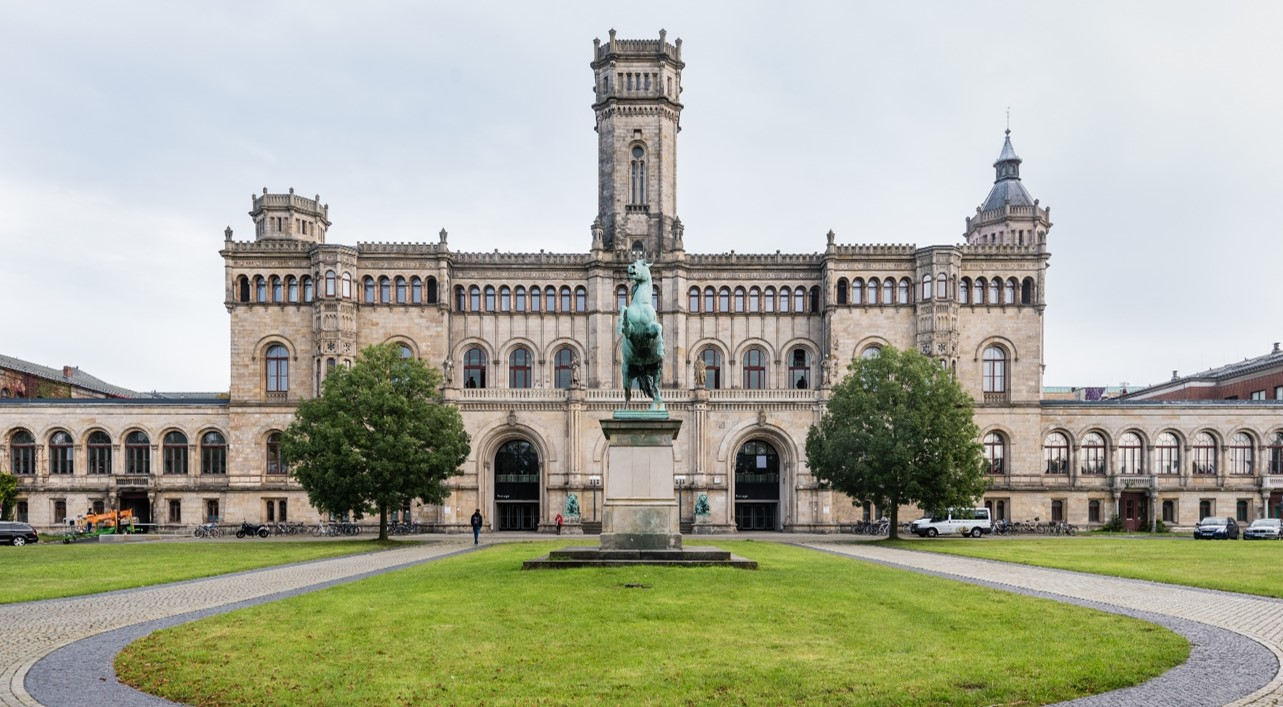
\includegraphics[width=0.75\textwidth]{figures/luh_default_presentation_title_image.jpg}}

\author[Abedjan \& Lindauer]{Ziawasch Abedjan \& Marius Lindauer\\[1em]
	
\includegraphics[height=\logoheight]{../latex_main/figures/luh_logo_rgb_0_80_155.pdf}\qquad
	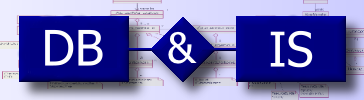
\includegraphics[height=\logoheight]{../latex_main/figures/DBIS_Kurzlogo.png}\qquad

\includegraphics[height=\logoheight]{../latex_main/figures/TNT_darkv4}\qquad

\includegraphics[height=\logoheight]{../latex_main/figures/L3S.jpg}	}
\date{Summer Term 2022; \hspace{0.5em} {
\includegraphics[height=1.5em]{../latex_main/figures/Cc-by-nc-sa_icon.svg.png}}; based on \href{https://ds100.org/fa21/}{[DS100]}
}


%%% Custom Packages
%----------------------------------------------------------------------
% Create dummy content
\usepackage{blindtext}

% Adds a frame with the current page layout. Just call \layout inside of a frame.
\usepackage{layout}


%%% Macros
%\renewcommand{\vec}[1]{\mathbf{#1}}
% \usepackage{bm}
%\let\vecb\bm

\title[Self-Supervised Learning]{DS: Learning}
\subtitle{Self-Supervised Learning}

\graphicspath{ {./figure/} }
%\institute{}


\begin{document}
	
    \maketitle
    
    \begin{frame}[c]{What is Self-Supervised Learning?}

        \begin{itemize}
            \item No labels $y_i$ are given at all
            \item Try to learn something about your $x$ distribution that can help for down-stream tasks\\ $\leadsto$ using an auxiliary or pretext task for that
            \item Example:
            \begin{itemize}
                \item Self-Supervised Learning step: remove patches from images and reconstruct these with a trained model $\leadsto$ only images $x_i$ are required for that
                \item Downstream task: Learn to predict an image classification model
            \end{itemize}
        \end{itemize}

    \end{frame}

    \begin{frame}[c]{Recovering of Missing Information}

        \begin{columns}
    
        \begin{column}{0.5\textwidth}
    
            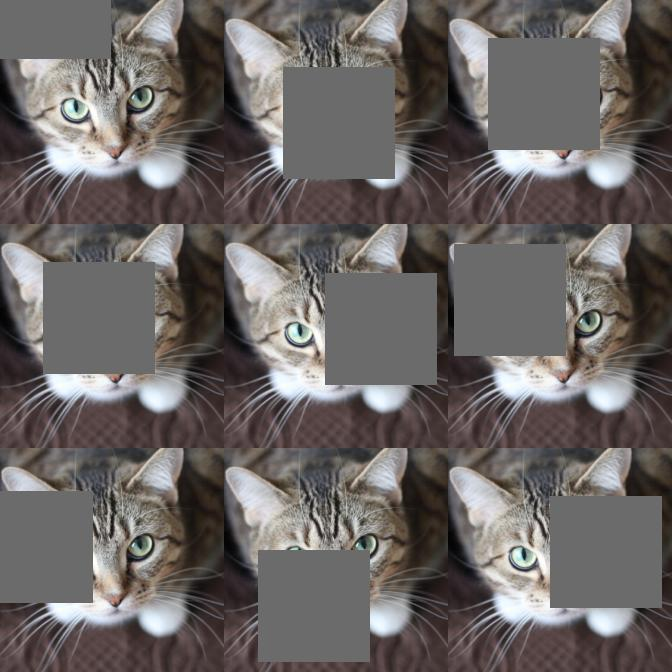
\includegraphics[width=0.75\textwidth]{figure/cutout.jpg}\\
            {\footnotesize \href{https://github.com/xkumiyu/numpy-data-augmentation}{[Source]}}
            
        \end{column}
    
        \begin{column}{0.5\textwidth}
    
            \begin{itemize}
                \item Learning to recover missing information from your input $x_i$ will help your model to learn a strong representation of your input data
                \item Simply set some of your features $x_i^{(j)} = 0$
                \item Vision Transformers (ViT) and LLMs based on transformers make use of this principle
            \end{itemize}
            
        \end{column}
    
        \end{columns}
    
        
    \end{frame}

    \begin{frame}[c]{Learning with Contrastive Loss}

        \begin{columns}
    
        \begin{column}{0.5\textwidth}
    
            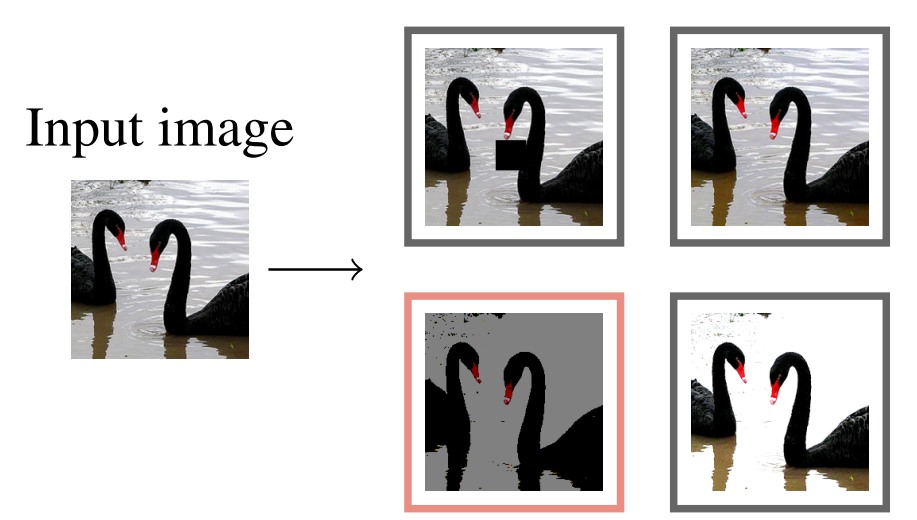
\includegraphics[width=0.9\textwidth]{figure/augmentation.png}
            
        \end{column}
    
        \begin{column}{0.55\textwidth}
    
            \begin{itemize}
                \item Learn which data points should be similar (without knowing labels of your data points~$x_i$)
                \item Use data augmentation to generate variations $x_i'$ of your input data $x_i$\\ $\leadsto$ you know that these two are somewhat similar
                \item learn with your model that $x_i$ and $x_i'$ are similar and dissimilar to other data points
                \begin{itemize}
                    \item the other data points can be sampled from your training data
                \end{itemize}
            \end{itemize}
            
        \end{column}
    
        \end{columns}
        
        
    \end{frame}

    
    \begin{frame}[c]{Exemplary Contrastive Loss Functions: Triplet loss}

        \alert{Triplet loss} is a commonly used loss function for learning embeddings, which is a type of representation that maps an input to a low-dimensional vector

            $$\max(0, d(x_A,x_P) - d(x_A,x_N) + \alpha)$$

            \begin{itemize}
                \item $x_A$ is an anchor sample (i.e., original data point $x_i$)
                \item $x_P$ is a positive sample (i.e., a sample that is similar to the anchor, e.g., by data augmentation)
                \item $x_N$ is a negative sample (i.e., a sample that is dissimilar to the anchor)
                \item $d(\cdot,\cdot)$ is the distance between two samples
                \item $\alpha$ is a margin that controls the distance between the anchor and negative samples
            \end{itemize}

         The goal of the triplet loss is to learn a representation of your data (i.e., an embedding), minimizing the distance between the anchor $x_A$ and positive sample $x_P$, while maximizing the distance between the anchor $x_A$  and negative sample $x_N$.
                
        
    \end{frame}

    \begin{frame}[c]{Downstream Tasks}

        \begin{itemize}
            \item For the downstream tasks, you have a few labeled data points -- often much less than for pure supervised learning
            \item A downstream task can be anything, incl. classification, regression, segmentation, \ldots
            \item \alert{Warning:} How well the downstream task can be learned can strongly depend on your self-supervised learning approach
        \end{itemize}
        
    \end{frame}

\end{document}